\documentclass[12pt]{article}
\usepackage{amsmath}
\usepackage{amsthm}
\usepackage{enumerate}
\usepackage{tikz}
\usetikzlibrary{shapes}
\newcommand{\mg} {\text{MG}_{\mathcal{G}}}

\title{Machine Learning in Complex Domains: Assignment 1}
\author{Ryan Cotterell, Dan Crankshaw, Dan Deutsch}

\begin{document}

\maketitle

\setcounter{section}{1}
\section{Problem Set}

\setcounter{subsection}{1}
\subsection{Designing an Extended Model}

Please see the {\tt network-extended.txt} and {\tt cpd-extended.txt} files for the
encoding of the model shown below.

\begin{center}
	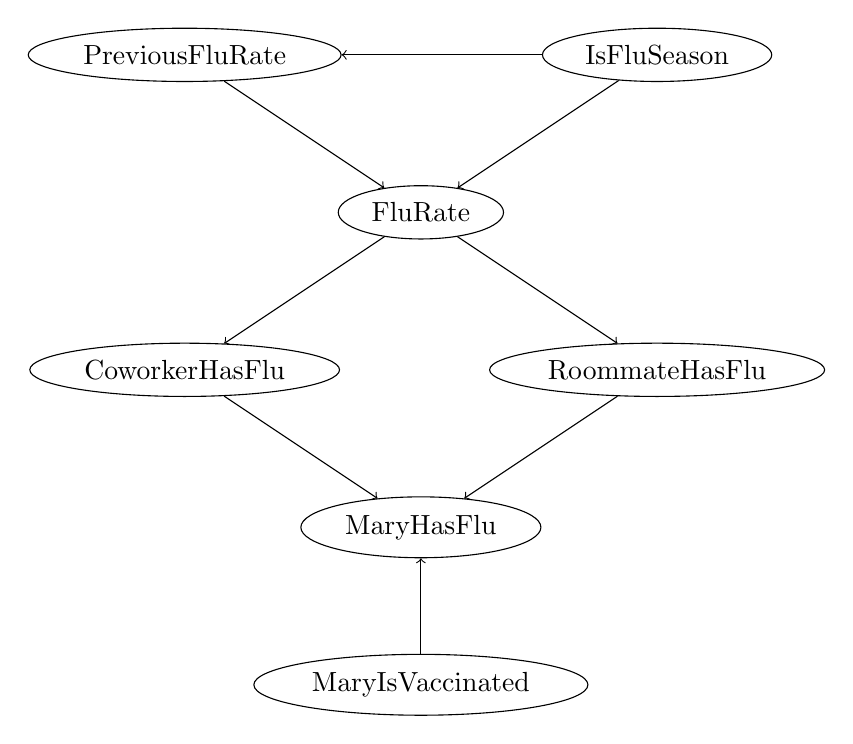
\begin{tikzpicture}

		\node (PreviousFluRate) at (0,8) [draw,shape=ellipse]{PreviousFluRate};		
		\node (IsFluSeason) at (6,8) [draw,shape=ellipse]{IsFluSeason};		

		\node (FluRate) at (3,6) [draw,shape=ellipse]{FluRate};		
		
		\node (CoworkerHasFlu) at (0,4) [draw,shape=ellipse]{CoworkerHasFlu};		
		\node (RoommateHasFlu) at (6,4) [draw,shape=ellipse]{RoommateHasFlu};				
		
		\node (MaryHasFlu) at (3,2) [draw,shape=ellipse]{MaryHasFlu};				
		
		\node (MaryIsVaccinated) at (3,0) [draw,shape=ellipse]{MaryIsVaccinated};						
		
		\draw [->] (IsFluSeason) -- (PreviousFluRate);
		\draw [->] (IsFluSeason) -- (FluRate);
				
		\draw [->] (PreviousFluRate) -- (FluRate);
		
		\draw [->] (FluRate) -- (CoworkerHasFlu);
		\draw [->] (FluRate) -- (RoommateHasFlu);
		
		\draw [->] (CoworkerHasFlu) -- (MaryHasFlu);
		
		\draw [->] (RoommateHasFlu) -- (MaryHasFlu);
		
		\draw [->] (MaryIsVaccinated) -- (MaryHasFlu);
	\end{tikzpicture}
	\end{center}
	
	
% PREVIOUS FLU RATE
\begin{center}
\begin{tabular}{|c|c|c|c|}
\hline 
 & \multicolumn{3}{|c|}{\textbf{PreviousFluRate}}  \\ 
\hline 
\textbf{IsFluSeason} & Mild & Moderate & Severe \\ 
\hline 
0 & 0.85 & 0.1 & 0.05 \\ 
\hline 
1 & 0.15 & 0.55 & 0.3 \\ 
\hline 
\end{tabular} 
\end{center}

% FLU RATE
\begin{center}
\begin{tabular}{|c|c|c|c|c|}
\hline 
\multicolumn{2}{|c|}{} & \multicolumn{3}{|c|}{\textbf{FluRate}} \\ 
\hline 
\textbf{PreviousFluRate} & \textbf{IsFluSeason} & Mild & Moderate & Severe \\ 
\hline 
Mild & 0 & 0.9 & 0.08 & 0.02 \\ 
\hline 
Mild & 1 & 0.2 & 0.5 & 0.3 \\ 
\hline 
Moderate & 0 & 0.4 & 0.55 & 0.05 \\ 
\hline 
Moderate & 1 & 0.1 & 0.65 & 0.25 \\ 
\hline 
Severe & 0 & 0.2 & 0.3 & 0.5 \\ 
\hline 
Severe & 1 & 0.1 & 0.3 & 0.6 \\ 
\hline 
\end{tabular} 
\end{center}

% COWORKER HAS FLU
\begin{center}
\begin{tabular}{|c|c|c|}
\hline 
 & \multicolumn{2}{|c|}{\textbf{CoworkerHasFlu}} \\ 
\hline 
\textbf{FluRate} & 0 & 1 \\ 
\hline 
Mild & 0.8 & 0.2 \\ 
\hline 
Moderate & 0.5 & 0.5 \\ 
\hline 
Severe & 0.2 & 0.8 \\ 
\hline 
\end{tabular} 
\end{center}

% ROOMATE HAS FLU
\begin{center}
\begin{tabular}{|c|c|c|}
\hline 
 & \multicolumn{2}{|c|}{\textbf{RoommateHasFlu}} \\ 
\hline 
\textbf{FluRate} & 0 & 1 \\ 
\hline 
Mild & 0.8 & 0.2 \\ 
\hline 
Moderate & 0.5 & 0.5 \\ 
\hline 
Severe & 0.2 & 0.8 \\ 
\hline 
\end{tabular}
\end{center} 

% MARY HAS FLU
\begin{center}
\begin{tabular}{|c|c|c|c|c|}
\hline 
\multicolumn{3}{|c|}{} & \multicolumn{2}{|c|}{\textbf{MaryHasFlu}}  \\ 
\hline 
\textbf{MaryIsVaccinated} & \textbf{RoomateHasFlu} & \textbf{CoworkerHasFlu} & 0 & 1 \\ 
\hline 
0 & 0 & 0 & 0.9 & 0.1 \\ 
\hline 
0 & 0 & 1 & 0.6 & 0.4 \\ 
\hline 
0 & 1 & 0 & 0.45 & 0.55 \\ 
\hline 
0 & 1 & 1 & 0.2 & 0.8 \\ 
\hline 
1 & 0 & 0 & 0.99 & 0.01 \\ 
\hline 
1 & 0 & 1 & 0.95 & 0.05 \\ 
\hline 
1 & 1 & 0 & 0.9 & 0.1 \\ 
\hline 
1 & 1 & 1 & 0.85 & 0.15 \\ 
\hline 
\end{tabular} 
\end{center}

\subsubsection{Model Properties}
\begin{enumerate}
	\item ``If Mary's roommate has the flu, Mary is more likely to catch the flu.''
	
	You can see in the CPTs above, whenever Mary's roommate has the flu, the probability
	that Mary has the flu increases compared to when her roommate does not have the flu.
	This also implies that Mary's roommate having the flu should be a parent of Mary getting
	the flu.
	
	\item ``Similarly, if Mary's coworker has the flu, Mary is more likely to catch the flu.''
	
	Similarly, the same situation applies as before: when Mary's coworker has the flu, the
	probability of Mary getting the flu increases. Again, this implies that Mary's coworker
	having the flu should be a parent of Mary getting the flu.
	
	\item ``Since Mary comes in closer contact with her roommate than her coworker, the
	probability of catching the flu increases more if her roommate has the flu than if
	her coworker has the flu. If both have the flu, then Mary is even likelier to catch it.''
	
	If you look at the CPT for {\bf MaryHasFlu},
	\begin{multline*}
		P(Mary = 1 \,|\, Roommate = 1, Coworker = 1, Vaccinated = 0) > \\
		P(Mary = 1 \,|\, Roommate= 1, Coworker = 0, Vaccinated = 0) > \\
		P(Mary = 1 \,|\, Roommate = 0, Coworker = 1, Vaccinated = 0)
	\end{multline*}
	and
	\begin{multline*}
		P(Mary = 1 \,|\, Roommate = 1, Coworker = 1, Vaccinaed = 1) > \\
		P(Mary = 1 \,|\, Roommate= 1, Coworker = 0, Vaccinated = 1) > \\
		P(Mary = 1 \,|\, Roommate = 0, Coworker = 1, Vaccinated = 1)
	\end{multline*}
	
	\item ``Mary's roomate and coworker are more likely to have the flu if the city's
	flu rate is elevated.''
	
	This statement implies that the flu rate should be the parent of both Mary's coworker
	getting the flu and Mary's roommate getting the flu. If you look at the CPTs for those
	nodes, as the flu rate gets more severe, the probability that they get the flu increases.
	
	\item ``If we know the flu status of Mary's roommate and coworker, then knowing the
	city's flu rate won't influence our belief about Mary catching the flu.''
	
	This implies that given Mary's roommate having the flu and Mary's coworker having
	the flu, Mary having the flu is independent of the city's flu rate. Therefore, the
	city's flu rate should not be connected to Mary has the flu, but should be the parents
	of Mary's coworker and Mary's roommate.
	
	\item ``Both the current flu rate and the flu rate two weeks ago are most likely to
	be mild if it is not currently the flu season. They are less likely to be moderate and 
	very unlikely to be severe.''
	
	This implies that the flu season should be parents of the current flu rate and the
	flu rate two weeks ago. If you look at the CPT for the flu rate, when it is not the flu season
	the probability that the flu rate is mild is greater than moderate which is greater
	than severe. Similarly the same is true for the previous flu rate.
	
	``If it is currently the flu season, then the flu rates are most likely to be moderate,
	followed by severe.''
	
	In all cases, when it is the flu season, the flu rates are most likely to be moderate, then
	severe, and finally mild.
	
	``The probability of being severe during the flu season is much higher than the same
	probability during the off season.''
	
	In all cases, the probability of the flu rates being severe is much greater when it is the
	flu season than when it isn't the flu season.
	
	\item ``The current flu rate in Mary's city is most likely to be the same level as the flu
	rate two weeks ago, since the flu rate typically does not change too rapidly. The next
	most likely level of the current rate depends on whether it is currently the flu season.''
	
	This condition contradicts some of the conditions imposed in the previous problem 
	because the previous problem states that if it is flu season, it is most likely moderate,
	severe, then mild. Then this problem says that they are more likely to be the same rate
	as the previous flu rate, which could pose a problem for when the last one was mild or
	severe. To make up for this, I tried to combine both and give slightly more probability
	to the previous flu rate. For example, if the last one was severe, then I shifted some of the
	mild and moderate probability to the severe column.

	\item ``Mary is less likely to catch the flu if she has been vaccinated for it this year.''
	
	In all situations if Mary is vaccinated, the equivalent probability of her getting the flu
	when she isn't vaccinated is larger than when she is vaccinated.

\end{enumerate}

\subsection{Network Manipulation}

Please see the {\tt network-F2.txt} and {\tt cpd-F2.txt} files for the encoding of our network.

\begin{center}
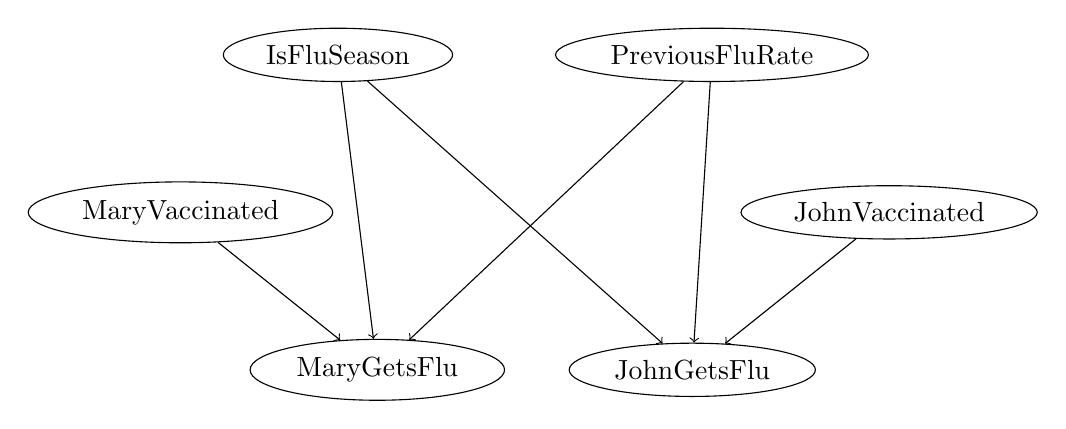
\begin{tikzpicture}

\node (MaryGetsFlu) at (2,0) [draw,shape=ellipse]{MaryGetsFlu};		
\node (JohnGetsFlu) at (6,0) [draw,shape=ellipse]{JohnGetsFlu};		
\node (MaryVaccinated) at (-.5,2) [draw,shape=ellipse]{MaryVaccinated};		
\node (JohnVaccinated) at (8.5,2) [draw,shape=ellipse]{JohnVaccinated};		
\node (IsFluSeason) at (1.5,4) [draw,shape=ellipse]{IsFluSeason};
\node (PreviousFluRate) at (6.25,4) [draw,shape=ellipse]{PreviousFluRate};				

\draw [->] (MaryVaccinated) -- (MaryGetsFlu);
\draw [->] (JohnVaccinated) -- (JohnGetsFlu);

\draw [->] (IsFluSeason) -- (MaryGetsFlu);
\draw [->] (IsFluSeason) -- (JohnGetsFlu);

\draw [->] (PreviousFluRate) -- (MaryGetsFlu);
\draw [->] (PreviousFluRate) -- (JohnGetsFlu);

\end{tikzpicture}
\end{center}

\begin{enumerate}

	\item The general procedure to take a graph $\mathcal{G}$, remove a node, $X_i$, and create
	an I-map, $\mathcal{G}'$ is the following. After $X_i$ is removed from the graph, you need
	to maintain the influence the parents of $X_i$ have on the children of $X_i$. For example,
	in the graph discussed in the problem, if we know nothing about \textbf{FluRate}, but we
	do know that it is the \textbf{FluSeason} and/or know something about the 
	\textbf{PreviousFluRate}, then that influences the probability of \textbf{MaryGetsFlu}.
	
	In order to maintain this relationship after $X_i$ has been removed, we need
	to connect the parents of $X_i$ to all of the children $X_i$. If one of those connections
	did not exist, we could infer from the graph that a parent and child of $X_i$ are independent,
	which we could tell from $\mathcal{G}$ that that assumption is not true. Therefore, if
	any of those connections are removed, it is creating an independence assertion that is not
	present in $\mathcal{G}$, and thus is not an I-map. So in order to create an I-map for
	$\mathcal{G}$, we need to connect all of the parents of the removed node, $X_i$ to all
	of the children of $X_i$.
	
	The probabilities for the new CPD can be attained as follows. Let $X$ be a node, $Y$ be the parent of that node we intend to remove and $Z_1,\ldots,Z_i$ be the parents of $Y$. We have the following CPDs $p(X|Y)$ and $p(Y|Z_1,\ldots,Z_i)$ By the chain rule, $p(X,Y|Z_1,\ldots,Z_i) = p(X|Y)p(Y|Z_1,\ldots,Z_i)$. Thus the new CPD for $X$ is
	$$
	P(X|Z_1,\ldots,Z_i) = \sum_{Y} p(X,Y|Z_1,\ldots,Z_i)
	$$
Thus we have attained a new minimal I-map, with a new CPD.
\end{enumerate}

\subsection{Network Queries}
Let's consider the sensitivity of a particular query $P(X|Y)$ to the CPD of a particular node $Z$.
Let $X$ and $Z$ be nodes (which are not directly connected) and Y be a set of nodes. We say that $Z$ has a requisite CPD for answering the query $P(X|Y)$ if there are two networks $\mathcal{B}_1$ and $\mathcal{B}_2$
that have identical graph structure $\mathcal{G}$ and identical CPDs everywhere except at the node $Z$, and
where $P_{\mathcal{B}_1}(X|Y) = P_{\mathcal{B}_2}(X|Y)$; in other words, the CPD of $Z$ affects the answer to this query.
This type of analysis is useful in various settings, including determining which CPDs we need
to acquire for a certain query.
Suppose we modify $\mathcal{G}$ into a graph $\mathcal{G}'$
which is identical to $\mathcal{G}$ except contains a new ``dummy''
node $\hat{Z}$ which is a parent of $Z$ (thereby altering the CPD of $Z$). One way to test whether $Z$ is
a requisite probability node for $P(X|Y)$ is to test whether $\hat{Z}$ has an active trail to $X$ given $Y$
in $\mathcal{G}'$ 	—if so, you can conclude that altering the CPD of $Z$ would affect the result of $P(X|Y)$. 

\subsubsection{Analytical Questions}
		Note. I am going to prove following as  discussed on Piazza. If $Z$ is found not to be requisite node, then again $P_{\mathcal{B}_1}(X|Y) = P_{\mathcal{B}_2}(X|Y)$, while if $Z$ is determined to be a requisite node, then there must exist at least one pair of networks such that $P_{\mathcal{B}_1}(X|Y) \not = P_{\mathcal{B}_2}(X|Y)$
\begin{enumerate}[1.]
	\item Prove that the above strategy is a sound criterion for determining whether $Z$ is a requisite probability node for $P(X|\mathbf{Z})$ in $\mathcal{G}$, that is, for all pairs of networks $\mathcal{B}_1,\mathcal{B}_2$, as $P_{\mathcal{B}_1}(X|\mathbf{Y}) \not = P_{\mathcal{B}_2}(X|Y)$ 
	\begin{proof}
	Suppose $Z$ is found not to be a requisite node. Thus by the definition of the criterion above there must not exist an active trail from $\hat{Z}$ to $X$. Thus there cannot exist an active trail from $Z$ to $X$. 
	
	We can prove that there is no from from $Z$ to $X$  by  contradiction. Suppose there was such a trail $T$ from $Z$ to $X$, then since $\hat{Z}$ is a parent of $Z$, we can extend $T$ with the edge from $Z$ to $\hat{Z}$ thus creating an active trail from $X$ to $\hat{Z}$, contradiction the criterion. 
	
	Thus by the definition of d-separation (as stated in the book), $X$ and $Z$ are conditionally independent. By the definition of conditionally independence $P_{\mathcal{B}_1}(X|Y) = P_{\mathcal{B}_2}(X|Y)$. So we conclude the criterion is valid.
	\end{proof}
	\item 
	Show that this criterion is weakly complete (like d-separation) in the sense that,
if it fails to identify $Z$ as a requisite in $\mathcal{G}$, there exists some pair of networks $\mathcal{B}_1$, $\mathcal{B}_2$ as before, $P_{\mathcal{B}_1}(X|Y) \not = P_{\mathcal{B}_2}(X|Y)$.
\begin{proof}
	Suppose $Z$ is found to be a requisite node. Thus by the definition of the criterion above, there must exist an active trail from $\hat{Z}$ to $X$. Thus there must exist an active trail from $Z$ to $X$ by the same reasoning above. Thus $Z$ and $X$ are \textit{not} d-separated. Thus by Theorem 3.4 in the book, $X$ and $Z$ are dependent given $\mathbf{Y}$ in some distribution. Let $\mathcal{B}_1$ a network in which the previous claim is true and let $\mathcal{B}_2$ be a network in which it is not true. Thus for these two networks $P_{\mathcal{B}_1}(X|Y) \not = P_{\mathcal{B}_2}(X|Y)$.
	\end{proof}
\end{enumerate}

\subsubsection{Empirical Questions}

\begin{enumerate}
	\item For the network in Figure 2, we let X=MaryGetsFlu, \textbf{Y} = MaryVaccinated, and
    Z = PreviousFluRate. For the network we designed, X=MaryGetsFlu, \textbf{Y} = FluRate,
    and Z=MaryIsVaccinated.\\

    \texttt{\$~~bayes-query network-F.txt data/cpd-F.txt MaryGetsFlu=Yes MaryVaccinated=Yes,PreviousFluRate=NotElevated
    0.05275}\\
    \texttt{\$~~bayes-query data/network-F.txt data/cpd-F.txt MaryGetsFlu=Yes MaryVaccinated=Yes,PreviousFluRate=Elevated
    0.143}\\\\

    \texttt{\$~~bayes-query data/network-extended.txt data/cpd-extended.txt MaryGetsFlu=Yes FluRate=Severe,MaryIsVaccinated=Yes
    0.1204}\\
    \texttt{\$~~bayes-query data/network-extended.txt data/cpd-extended.txt MaryGetsFlu=Yes FluRate=Severe,MaryIsVaccinated=No
    0.668}\\

	\item For the network in Figure 2, X=MaryGetsFlu, \textbf{Y} = FluRate, Z=PreviousFluRate.
    For the network we designed, X = MaryGetsFlu, \textbf{Y} = FluRate, Z = IsFluSeason.\\

    \texttt{\$~~bayes-query data/network-F.txt data/cpd-F.txt MaryGetsFlu=Yes FluRate=Elevated,PreviousFluRate=Elevated 
    0.35}\\
    \texttt{\$~~bayes-query data/network-F.txt data/cpd-F.txt MaryGetsFlu=Yes FluRate=Elevated,PreviousFluRate=NotElevated
    0.35}\\\\
    \texttt{\$~~bayes-query data/network-extended.txt data/cpd-extended.txt MaryGetsFlu=Yes FluRate=Severe,IsFluSeason=Yes
    0.3942}\\
    \texttt{\$~~bayes-query data/network-extended.txt data/cpd-extended.txt MaryGetsFlu=Yes FluRate=Severe,IsFluSeason=No
    0.3942}\\


\end{enumerate}

\subsection{Markov Blankets and D-Separation}
Let $\text{MB}_{\mathcal{G}(X)}$ denote the Markov blanket of node $X$ in an \textbf{undirected} graph $\mathcal{G}$, whose set of nodes is denoted $\mathcal{X}$. The Markov blanket of $X$ is the set of $X$'s neighbors. 
\begin{enumerate}[1.]	
	\item 
	\begin{enumerate}[(a)]
		\item For any variable $X$, let $\mathbf{W} = \mathcal{X} - \{X\} - \text{MB}_{\mathcal{G}}(X)$. Then $X$ and $\mathbf{W}$ are d-separated given $\text{MB}_{\mathcal{G}}(X)$
		\begin{proof}
		Suppose by way of contradiction that $X$ and $\mathbf{W}$ were not d-separated given $\text{MG}_{\mathcal{G}}(X)$. Thus by the definition d-separation, there must be an active trail $T$  from a node $w\in \mathbf{W}$ to $X$. $X$ and $w$ are not adjacent since all all nodes adjacent to $X$ are in $\text{MG}_{\mathcal{G}}(X)$ since by construction $w$ is not in $\text{MG}_{\mathcal{G}}(X)$. So it follows that there must exist an element $m \in \text{MG}_{\mathcal{G}}(X)$ that is also in trail $T$ since the trail must begin with $X$ and advance to an adjacent node. Since $m$ is observed, this contradicts the definition of an active trail.
		\end{proof}
	\item The set $\text{MG}_{\mathcal{G}}(X)$ is the minimal set for which this property holds. 
		\begin{proof}
		Suppose by way of contradiction that $\mg(X)$ is not the minimal set for which this property holds. This implies we can remove a node from $\mg(X)$ and the property will still hold. Let $y$ be an arbitrary node in $\mg(X)$. We then remove $y$ from $\mg(X)$. Since $y$ was in $\mg(X)$,  $y \in N_\mathcal{G}(X)$. By the definition of a neighborhood, there exists a vertex $v$ from $X$ to $y$.  Let $T = (X, v, y)$ be a trail. Since no node on $T$ is observed, $T$ is active. Additionally, since no node in $\mg(X)$ is on $T$, $T$ remains active if every element in $\mg(X)$ in observed. This contradicts the assertion 2.5.1a proved above since $y$ is therefor in $\mathbf{W}$ and thus $X$ and $\mathbf{W}$ are not d-separated given $\mg(X)$
		\end{proof}
	\end{enumerate}
	\item 
			Now suppose that $\mathcal{G}$ is directed. In a directed graph, the Markov blanket of $X$ is the following set of nodes: $X$'s parents, $X$'s children, and $X$'s children’s parents. We would like to prove the two statements in question 1 above in the directed case. It turns out that you can do this straightforwardly by utilizing the proofs you have already constructed for the undirected case. Please sketch a proof of these two statements for a directed graph $\mathcal{G}$ which relies on the proof for the undirected case. Your answer should be brief if your solution is complicated, you are probably on the wrong track.
\begin{proof}
Let $\mathcal{G}$ be an directed graph. For any variable $X$, let $W = \mathcal{X} - \{ X\} - \mg(X)$. 
Let $\mathcal{M}[\mathcal{G}]$ be the moral graph of a the Bayesian network $\mathcal{G}$ (Definition 4.16). That is by definition there is an an undirected edge between nodes $X$ and $Y$ in $\mathcal{G}$ if there is a directed edge between them or they are both parents of the same node. By the definition of a Markov Network, $\mathcal{M}[{\mathcal{G}}]$ is a Markov network and additionally $\mathcal{M}[\mathcal{G}]$ is a minimal I-map for $\mathcal{G}$. Now to prove the claim we simply need to show that the  all $X$'s neighbors in $\mathcal{M}[\mathcal{G}]$ corresponds to $X$'s parents, $X$'s children and $X$'s childrens parents. The the definition of the transform $\mathcal{M}$ undirected edges exist wherever a directed edge exists so $X$'s parents and $X$'s children are connected to $X$ by undirected edges. Additionally, there must be an undirected edge between $X$'s childrens parents since $X$ and a parent of one of $X$'s children are parents of a shared node, namely one of $X$'s children. Thus $X$'s parents, children and children's parents are all neighbors of $X$ in $\mathcal{M}[\mathcal{G}]$ so they are all in $\mg(X)$ in $\mathcal{M}[\mathcal{G}]$. Since $\mathcal{M}[\mathcal{G}]$ is a Markov Network, the proves from 2.5.1 hold and we have proved the claim.
\end{proof}

\end{enumerate}
\subsection{Comparing Network Types: Disease severity over time}
In this section, we will consider modeling the severity of a disease over time using linear chain graphical models, which are commonly used to model discrete time series data.
The random variable $Y_i$ denotes the disease severity (None, Mild, Severe) on day $i$. The random variable $S_{i,j}$ indicates a symptom $j$ on day $i$, such as the patient’s temperature or whether or not she has a cough (for example, if Mary had a case of the flu, we could model it day-by-day using such a model). The symptoms $\mathbf{S}$ are observed. The severity $\mathbf{Y}$ is not observed, but it can be inferred from the observed symptoms.
Figure 3 shows three different types of networks to model this. The first is directed graph which encodes $P(\mathbf{Y}, \mathbf{S})$, called a hidden Markov model (HMM). The second is a directed graph which encodes $P(\mathbf{Y}|\mathbf{S})$ called a maximum-entropy Markov model (MEMM). The third is a type of conditional random field (CRF), which also models $P(\mathbf{Y}|\mathbf{S})$. CRFs can be partially directed or undirected; a partially directed version is shown here.
The differences between these models are subtle, and even in practice it is not always clear which model to use. As you’ll learn later in the semester, the choice of model has implications and tradeoffs regarding learning and inference. In this assignment, we want you to think about the subtle differences in assumptions made by these models.
\subsubsection{Analytical Questions}

\begin{enumerate}[1.]
	\item 
		\begin{enumerate}[(a)]
			\item HMM = Yes, MEMM = No, CRF = Yes
			\item HMM = No, MEMM = Yes, CRF = No
			\item HMM = No, MEMM = No, CRF = No
		\end{enumerate}
		By the test in 2.4
	\item \begin{enumerate}[(a)]
		\item
				First of all, given that there are a lot of features, we have to take computational cost into account. In that regard, HMMs and MEMMs are much easier to learn, where as training a CRF can be computationally prohibitive. Second of all, we come to the age-old problem of generative models versus descriminative models. HMMs are generative whereas MEMM and CRFs are descriminative. Therefore the HMM will attempt to model $p(x,y) = p(y|x)p(x)$. In many cases modeling $p(x)$ is extremely hard as we have to explicitly model the features and the interactions between them. Given the amount of in domain knowledge we have, we may or may not want to go for a generative model. If we can model $p(x)$ reasonably well, it is  better to go with a generative model because it is often   possible to learn with less data. The discriminative models , MEMM and CRF, are both useful when, we can't explicitly model $p(x)$. The label bias problem makes  MEMM a poor choice.  MEMMs make an independence assumption (see 2.6.1.a) between time steps. This means that a later observations has no affect on previous observations. For this reason MEMM are generally avoided in favor of CRFs despite, the computational cost of training a CRF.	
				\item I want to clarify that I am going to answer this question about feature correlation at a given time step. Feature correlation is not a problem for discriminative models in general because are a not modeling the features. This means that we don't really need to worry about feature correlation in the discrimination model. For the HMM, we need to accurately model the features and their independence assumptions. If we do this incorrectly, such as assuming independence, we could violate independence assumptions. 
	\end{enumerate}
\end{enumerate}
\subsection{Noisy-OR  other possible causes.}
	\subsubsection{Analytical Questions}
	One property of Bayesian networks is something called \textit{explaining away }which occurs when
evidence that establishes a cause for an event reduces the likelihood of
		\begin{enumerate}
			\item	
				\begin{enumerate}[(a)]
					\item Show that this network must satisfy the explaining-away property $P(x^1|z^1) \geq P(x^1|y^1,z^1)$
					\begin{proof}
					\begin{eqnarray*}
						p(x^1|z^1,y^1) &=& \frac{p(x^1,y^1,z^1)}{p(z^1,y^1)} \\
												&\leq & \frac{p(x^1,y^1,z^1) + p(x^1,y^0,z^1)}{p(z^1,y^1) + p(x^1,y^0,z^1)}\; \text{By the Mediant inequality} \\
												&\leq & \frac{p(x^1,z^1)}{p(z^1,y^1) + p(x^1,y^0,z^1)} \\
												&\leq & \frac{p(x^1,z^1)}{p(z^1,y^1) + p(x^1,y^0,z^1) + p(x^0,y^0,z^1)}\; \text{note that } p(x^0,y^0,z^1) = 0 \\
												&\leq & \frac{p(x^1,z^1)}{p(z^1,y^1) + p(z^1,y^0)} \\
												&\leq & \frac{p(x^1,z^1)}{p(z^1)} \\
												&\leq & p(x^1|z^1)
					\end{eqnarray*}
					This shows that $p(x^1|z^1,y^1) \leq p(x^1|z^1)$. \\
					Note that I continued to the $\leq$ on the right hand side to indicate that the right hand size is less than the original left hand size equation. All of the left hand side equations after the first are in fact equivalent. 
					\end{proof}
						\item 
							\begin{tabular}{c||c c c c}
								$Z$ & $x^0,y^0$ & $x^0,y^1$ & $x^1,y^0$ & $x^1,y^1$  \\ \hline
								$z^0$ & .9 & .9 & .9 &  .1 \\
								$z^1$ & .1  & .1 & .1 & .9
							\end{tabular} \\
							
						Additionally, we assume that no probability can be 0. Without this assumption the claim is not true since $p(y^1)$ could = 0, which would invalidate the inequality $p(x^1|z^1,y^1) > p(x^1|z^1)$. We can only prove the weaker claim of less than or equal to one. We also assumed a uniform prior since this would allow us to show this through our program.
						\begin{verbatim}
						./bayes-query network-Test.txt cpd-Test.txt X=1 Z=1,Y=1
0.9
						./bayes-query network-Test.txt cpd-Test.txt X=1 Z=1
0.833333333333
						\end{verbatim}
						\item $p(x^1|y^0,z^0) = p(x^0|y^1,z^0)$, that is that $x$ is conditionally independent of $y$ given $z=0$. This makes sense because there is no longer an effect effect that two causes are competing to explain. 
					\end{enumerate}
				\item 
					\begin{enumerate}[(a)]
							\item For each $D_m$, such that $\ell < m \leq k$. For each child of $D_m$, marginalize over its CPD by summing over all values the random variable $D_m$ can take. 
							\item No, we won't get the an exact transformation. The random variables we have eliminated no longer serve as valid causes for the symptoms. We have just averaged out their effects so we can no loner ascribe symptoms to them.						
			
					\end{enumerate}
		\end{enumerate}
        \subsubsection{}
        \begin{enumerate}
        \item
        We can construct the new \emph{noisy or} CPD for $F_i$ using the node elimination
        algorithm we created in section 2.3. We essentially just marginalize over the
        $D_i$ that we are eliminating to create the new CPD\@. The original CPD for
        node $F_i$ is:
        \begin{equation*}
            P(f_i^0 | \boldsymbol{Pa}_{F_i}) = (1 - \lambda_{i,0}) \prod_{D_J \in \boldsymbol{Pa_{F_i}}} (1 - \lambda_{i,j})^{d_j}
        \end{equation*}

        To create the new CPD we perform the following operation for each $D_m$
        where $l < m < k$:
        \begin{align*}
                P(f_i^0 | \boldsymbol{Pa}_{F_i} - {D_m}) & =
                P(f_i^0 | \boldsymbol{Pa}_{F_i} - {D_m}, D_m = 0) P(D_m = 0)\\
                & + P(f_i^0 | \boldsymbol{Pa}_{F_i} - {D_m}, D_m = 1) P(D_m = 1)\\
                & = (1 - \lambda_{i,0})(1-\lambda_{i,m}) P(D_m = 1) \prod_{D_J \in \boldsymbol{Pa_{F_i}} - {D_m}} (1 - \lambda_{i,j})^{d_j}\\
                & + (1 - \lambda_{i,0}) P(D_m = 0) \prod_{D_J \in \boldsymbol{Pa_{F_i}} - {D_m}} (1 - \lambda_{i,j})^{d_j}
        \end{align*}
        This procedure will eliminate each of the unneeded parents without changing the joint
        transformation over $D_i, \ldots, D_l, F_i$.
        \item
        This is an exact algorithm and will thus yield an exact transformation. We will
        get the correct posterior probability relative to the original model with the
        transformed model as well because in order to calculate the posterior probability
        we would have to marginalize over the other $D_i$ anyway.
        \end{enumerate}




\end{document}
